\section{Analysis of results}

\todo{This section needs significant revision.}

\subsection{Batch Query Evaluation}
In case of batch query evaluation, both OCL implementations use the same
algorithm, thus their execution time is roughly the same. The roughly negligible
differences are due to the initialization of the OCL Impact Analyzer.

For the \emph{batch query} evaluation of the \textsf{RouteSensor} query
\autoref{fig:BatchValid_RouteSensor} shows that \eiq{} performs similarly
to Eclipse OCL. It is slightly faster for small models (2 s and 3 s
respectively), but is slower for large models (up to 125 s and 78 s), where
this 50\% slowdown (once in the whole scenario) can be attributed to the
initial (Rete) cache build.

% Both OCL measurements use Eclipse OCL for the batch phase,
% because the Impact Analyser is not built for this purpose according to the
% authors. However, the initialisation of the OCL Impact Analyser also occurs in
% this phase resulting in (roughly negligible) higher execution time.

% \begin{figure}[ht]
% \begin{center}
% 	\begin{subfigure}[t]{0.48\textwidth}\centering
% 	    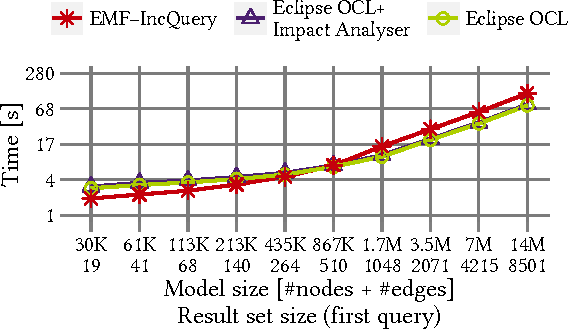
\includegraphics[width=0.9\textwidth]{figures/trainBenchmark_User_BatchValid_RouteSensor}
% 	    \caption{Batch Query Evaluation Time -- RouteSensor}
% 	    \label{fig:BatchValid_RouteSensor}
% 	\end{subfigure}
% 	\begin{subfigure}[t]{0.48\textwidth}\centering
% 	    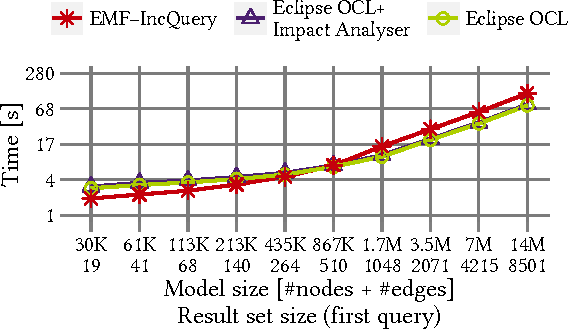
\includegraphics[width=0.9\textwidth]{figures/trainBenchmark_User_BatchValid_RouteSensor}
% 	    \caption{Batch Query Evaluation Time -- SignalNeighbor}
% 	    \label{fig:BatchValid_SignalNeighbor}
% 	\end{subfigure} \\
% 
% 	\begin{subfigure}[t]{0.48\textwidth}\centering
% 	    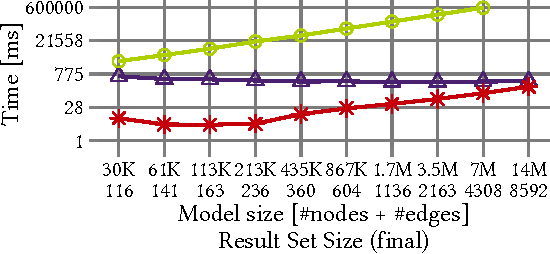
\includegraphics[width=0.9\textwidth]{figures/trainBenchmark_User_SumInc_RouteSensor}
% 	    \caption{Incremental Query Evaluation Time -- RouteSensor}
% 	    \label{fig:SumInc_RouteSensor}
% 	\end{subfigure}
% 	\begin{subfigure}[t]{0.48\textwidth}\centering
% 	    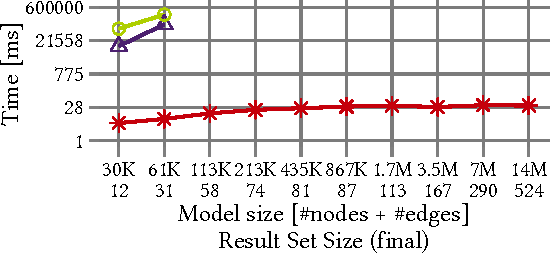
\includegraphics[width=0.9\textwidth]{figures/trainBenchmark_User_SumInc_SignalNeighbor}
% 	    \caption{Incremental Query Evaluation Time -- SignalNeighbor}
% 	    \label{fig:SumInc_SignalNeighbor}
% 	\end{subfigure} \\
% 
% 	\begin{subfigure}[t]{0.48\textwidth}\centering
% 	    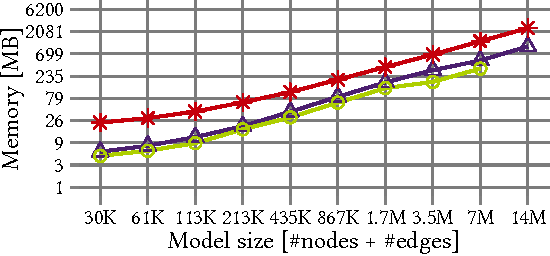
\includegraphics[width=0.9\textwidth]{figures/trainBenchmark_User_Memory_RouteSensor}
% 	    \caption{Memory Usage -- RouteSensor}
% 	    \label{fig:Memory_RouteSensor}
% 	\end{subfigure}
% 	\begin{subfigure}[t]{0.48\textwidth}\centering
% 	    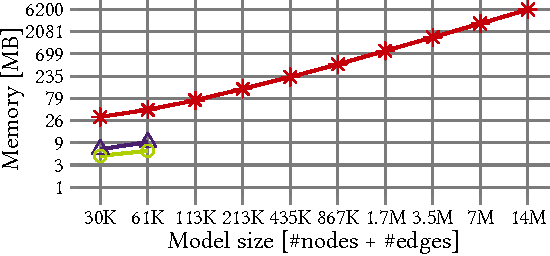
\includegraphics[width=0.9\textwidth]{figures/trainBenchmark_User_Memory_SignalNeighbor}
% 	    \caption{Memory Usage -- SignalNeighbor}
% 	    \label{fig:Memory_SignalNeighbor}
% 	\end{subfigure}
%   \caption{Benchmark results.}
%   \label{fig:trainbenchmark-diagrams}
% \end{center}
% \end{figure}

For the more complex \textsf{SignalNeighbor} query
\autoref{fig:BatchValid_SignalNeighbor} depicts that \eiq{} (somewhat
surprisingly) outperforms OCL solutions: it is noticeably faster for small
modells (2 s and 4 s), and over 435k model elements OCL did not finish with
the initial analysis in 12 minutes. This performance gain might be attributed to
the more efficient (cached) enumeration of instances, and the possibility of
backward navigation (with the help of auxiliary structures) on unidirectional
references used by this query.

\subsection{Incremental Query Evaluation}
In the \emph{incremental case}, Eclipse OCL evaluates the query on each run
(100 times) from scratch, its execution time increases linearly with
model size, resulting slow overall evaluation.

For the \textsf{RouteSensor} query (\autoref{fig:SumInc_RouteSensor}), the Impact
Analyzer performs the 100 modifications in 350 ms regardless of the model
size. On the same query, \eiq{} starts much faster, but its speed reduces
on the larger models (from 9 to 220 ms). On the other hand, the Impact
Analyzer is an order of magnitude slower on the \textsf{SignalNeighbor} query
(\autoref{fig:SumInc_SignalNeighbor}) query: it does not finish in 12 minutes
for models over 61k model elements, while \eiq{} handles every model
regardless of size under 40 ms.

The performance of the Impact Analyzer is most likely affected by the previously
mentioned unidirectional references. The slowdown of \eiq{} is probably
caused by the increased number of matches (from 116 to 8592), as query
results are always available in the output nodes of Rete networks, and only a
linear traversal of these stored matches is needed to return them.

\subsection{Threats to Validity}
We tried to mitigate \emph{internal validity} threats by reducing the number of
uncontrolled variables during measurements: a physical machine was used with all
unnecessary software components turned off and every execution was isolated into
a freshly initialized JVM.

The queries are semantically equivalent in the different query languages and the
result sets are the same for every model. Additionally, to ensure comparable
results the created high-quality query implementations were reviewed: the OCL
implementation by Ed Willink from the Eclipse OCL project, the usage of Impact
Analyzer by Axel Uhl from the Impact Analyzer developer team. The graph patterns
were written by the developers of \eiq{}.

Considering \emph{external validity}, the generalization of the results largely
depends on how representative the metamodels, the models and the queries are
compared to real use cases. In section \ref{specification-extended} metrics were
defined to describe complexity of models and queries, however comparing them to
real world ones remains a future work.

The metamodel and the query specifications were motivated by an industrial case
study, and the selected queries feature commonly used validation tasks such as
attribute and reference checks or cycle detection. We tried to ensure that the
instance models have a similar structure and distribution to other models by
parameterizing the generation process based on our experience with other
domains. To summarize, we believe that the train domain and the generated
instance models represent other domain-specific languages and available instance
models well.

Our current measurements only loaded and executed a single query in each run.
When loading multiple queries, query interference may change the results
greatly. A more detailed evaluation of this issue is planned for the future.

Considering resource-constrained environments, we believe that limiting
available memory will alter the results the most, as the memory management
overhead will reduce the performance of \eiq{}.

It is important to note that heap usage were measured after executing a garbage
collection, so these measurements do not contain memory usage of temporary
constructs. This means that maximum heap usage might have been larger. Furthermore,
limiting heap space by the maximum usage results in excessive garbage collection
and thus an increased runtime. However, in our experience setting the limit to
two times the measured values, such issues do not occur.

In case of the benchmark queries, we measured a $1.5$GB heap size in case of a
model with $3.5$M model elements that we believe is manageable in a developer
machine with $4$--$8$GB of RAM. On the other hand, when handling such large
models the existing user interface itself could become a bottleneck. Thus we
believe, our measurement results hold also in the integrated development
environments.
